

%{\normalfont\initfamily \fontsize{12mm}{12mm}\selectfont D}
\cappar Si el esfuerzo sin talento, sirve de poco, el talento sin trabajo sirve de nada, sino para inspirar lamento por el desperdicio. En ajedrez, como en tantos artes, como en la vida, las horas de estudio y vuelo aportan un plus difícil de lograr por otras vías. Pero para revolucionar, innovar o causar sensación, es casi imprescindible ser un tarado, un tipo dedicado prácticamente en exclusividad a ello, en el que el dia y la noche la cabeza gira hacia el mismo objetivo.

Hay ejemplos antagónicos, tipos bendecidos por la varita de la genialidad que sin embargo permanecían aparentemente ajenos a su entorno. De Ronaldo, el bueno, el brasileño gordito, saltaba al Bernabeu sin saber muchas veces quien era el rival. De Garrincha el equilibrista divino de la gambeta, saltó al campo en una copa del mundo y preguntó sorprendido porque había un ambiente tan tremendo en las gradas, „Es la final“, le contestaron. O Best, otro brillante que usó su magia para conseguir su gran pasión „la dolce vita“.

Negreanu „the Kid“ instauró un antes y un después en el mundo de Holdem, descabalgando un universo estático monopolizado por dinosaurios y popularizó un juego ancestralmente reservado a tiburones y pardillos.  

Guardiola perfeccionó un estilo, e innovo una forma de desarrollo, quizás la más plástica y estética que jamás hubo. En ambas biografías se destaca su obsesión patológica por sus disciplinas, los estudios sesudos, horas gratuitas, muchas veces infructuosas de observación, experimentación, e infinitos análisis. Ensayo-error enfrascados en su realidad paralela como becarios de laboratorio haciendo méritos.

Miguel Illescas, GM y pedagogo, modelo y espejo de varias generaciones de aficionados hispanos se lamenta profundamente de unos años preciosos, de los 13 a los 18 en los que no pudo dedicarse más intensamente al ajedrez y que le mermaron a posteriori, impidiendo llegar a ser mucho más.

Actualmente, las circunstancias han cambiado. Irrumpen chavales cada vez más jóvenes en los altos niveles. Situación anteriormente impensable. La juventud tiene la ventaja de la mente fresca, la inquietud intacta, desconocer los sinsabores, las ansias de vida, la rapidez de ejecución, una mayor resistencia, pero carece de experiencia. 

\begin{wrapfigure}{r}{0.55\textwidth} 
 \begin{figurebox}
       \centering
   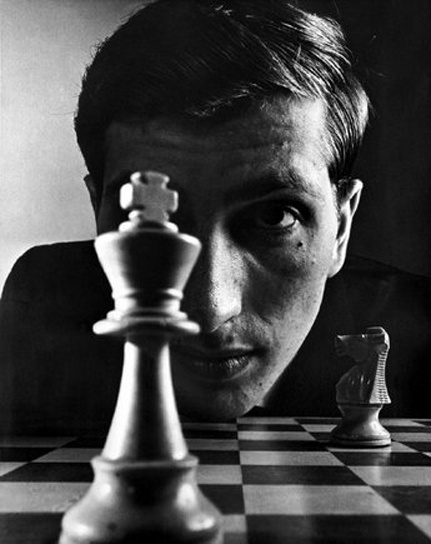
\includegraphics[scale=0.45]{ajedrez.jpg}
  \end{figurebox}
\vspace{-0.5cm}
\end{wrapfigure}

Internet cambió radicalmente las reglas. A golpe de click todo el mundo tiene acceso sencillo a un universo infinito, de prácticas, de herramientas, artículos, colecciones de partidas, blogs al respecto, libros de todos los elementos de cada disciplinas. Uno puede sumar tantas horas de estudio como disponga y deseé. 

Y se da la paradoja que algún veinteañero enajenado, un yihaidista del blanco y negro haya disfrutado de tantas partidas como un GM que le dobla la edad. Si a eso le mezclamos, en el tubo de ensayo, la agilidad de unas neuronas con recorrido  y las ansias de gloria y parné se consigue una solución dinamitera: Éxito brutal.

Solo así, a partir de años horas y entusiasmo robadas a otras actividades propias de su etapa evolutiva, a base de juventudes extraviadas, se explican las mesas finales de torneos de poker repletas de barbilampiños, y la llegada de probablemente el mejor jugador de la historia del ajedrez con la insospechada edad de 22 años. Un tipo que por si mismo no merece un post, sino un libro, o varios

Actual campeón del mundo en las tres modalidades, o sea el mejor, sin discusión, en cualquier circunstancia. Con una visión intuitiva, dinámica, máquinal, casi eléctrica, forjada a base de pantalla, de libros, de artículos, de bibliotecas de partidas, de exámenes contrastados con el ordenador, de debates con semejantes.

Una corta vida entrelazada en piezas de marfil, apetito insaciable por descifrar la diagonal escondida, el travieso desliz, el acertijo diario del periodico, un tibetano en sus montañas de alfiles de espaldas al mundo.

Lo que ha personalizado Carlson, en su bisoñez, es un sinsentido, una realidad incapaz de alcanzarse si no se parte como hizo el demente noruego desde el exacerbado fanatismo que practica y que le ha atajado más allá de la excelencia.

Su limite llegará el día en el que el tema, quizás por no encontrar un rival a su altura, o por haber saciado bolsa y olimpo, deje de interesarle.


%\begin{wrapfigure}{r}{0.35\textwidth} 
  \vspace{1.5cm}
%  \begin{figurebox}
%    \vspace{20pt}
   \centering
   
\includegraphics[scale=0.4]{aihbbgje.jpg}\\
%    Enrique Luis Ibáñez Conde\\ 
%    Diretor executivo\\
%    {\sl SAEMA Projectos na área
%      eléctrica e médica, LDA}
%    %\vspace{0.1\textheight}
%  \end{figurebox}
%  \vspace{-10pt}
%
%\end{wrapfigure}


\newpage
%%% Local Variables: 
%%% mode: latex
%%% TeX-master: "nadaesimposible"
%%% End: 


